\chapter{Příklady kontrolních programů}
\label{priklady}

Velmi důležitou součástí dokumentace knihovny je ukázka jejího použití pro
vyřešení komplexního problému. Samotný popis jednotlivých metod většinou
nestačí uživateli k napsání vlastního programu. Je potřeba předvést jak se
knihovna používá od vzniku programu až do jeho ukončení.

Záměrem této práce není pouze vytvořit knihovnu pro ovládání robota, ale také
předvést k čemu se dá robot použít a ukázat jak lze řešit některé časté úkoly.
Proto v této kapitole bude k nalezení hned několik kompletních programů
demonstrujících vlastnosti e-puck robota a použití e-puck knihovny.

Účelem ukázkových programů není uživatelům diktovat jakým způsobem mají
využívat knihovnu. Jde pouze o inspiraci. Jak bude vidět, tak některé ukázkové
programy řeší ovládání velmi odlišně. Po přečtení by však kdokoli znalý
programování měl být schopen velmi rychle napsat ovládací program dle svých
představ.

\section{Braitenberg Vehicle}
\label{braitenberg vehicle}

Braitenberg vehicle je experiment provedený italsko-australským vědcem
Valentinem Braitenbergem. Zkoumal evoluční vývoj jednoduchých agentů a
senzoricko-motorické interakce mezi robotem a prostředím, bez potřeby vnitřní
paměti nebo reprezentace prostředí.

V elementární formě jsou senzory přímo napojeny na akční členy. Například
naměřené hodnoty světla na senzorech ovlivňují rychlost motorů. Robot pak může
vykazovat i pomocí triviálního programu na první pohled komplexní chování.
Pokud má robot dva senzory a dvě kola a ty jsou spolu propojeny tak, že levý
senzor zvyšuje rychlost levého kola se zvyšující se intenzitou a naopak pravý
senzor zvyšuje rychlost pravého kola se snižující se intenzitou, pak robot může
vykazovat komplexní chování ve chvíli, kdy bude kroužit okolo zdroje světla.

\subsection{Zdrojový kód}

Ukážeme si trochu komplikovanější program, který se, v závislosti na senzorech
překážek, snaží s robotem uhýbat překážkám. Program je o něco delší, protože
je potřeba normalizovat hodnoty na vstupech a upravit podle nich rychlost
motorů.

\begin{mylisting}
\begin{pyc}
#!/usr/bin/env python
# -*- coding: utf-8 -*-

import logging
import time
import signal
import sys

from epuck import Controller, WrongCommand

c = Controller('/dev/rfcomm0', asynchronous=True)

bias = 200
too_close = 2000
max_speed = 1000
min_speed = -1000

# Signal handler to cleanup after shutdown
def handle_signal(signum, frame):
    r = c.set_speed(0,0)
    r.join()
    sys.exit(0)

# SIGINT is interrupt signal sent by CTRL+C
signal.signal(signal.SIGINT, handle_signal)

while True:
    # Read values from proximity sensors
    r = c.get_proximity_sensors()
    r = r.get_response()

    left_sensors = r['L10'] + r['L45'] + r['L90'] + bias
    right_sensors = r['R10'] + r['R45'] + r['R90'] + bias

    left_speed = left_sensors if right_sensors < too_close \
                 else -left_sensors
    right_speed = right_sensors if left_sensors < too_close \
                  else -right_sensors

    if left_speed > max_speed: left_speed = max_speed
    if left_speed < min_speed: left_speed = min_speed
    if right_speed > max_speed: right_speed = max_speed
    if right_speed < min_speed: right_speed = min_speed

    try:
        c.set_speed(left_speed, right_speed)
    except WrongCommand:
        pass

    time.sleep(0.1)

\end{pyc}
\captionof{listing}{Program pro robota, který se snaží vyhýbat překážkám.}
\label{braitenberg}
\end{mylisting}

\subsection{Vysvětlení programu}

Rozebereme si nyní program. Je třeba předeslat, že struktura programu je velmi
jednoduchá. Použít pro ovládání robota nekonečnou smyčku je tradiční řešení,
měl by ovšem existovat způsob, jak robota zastavit. Tady se jedná o
interaktivní řešení, kdy robota může zastavit uživatel zasláním přerušení
SIGINT (zmáčknutí CTRL + C).

Ve zdrojovém kódu \ref{sigint handler} vytváříme metodu \code{handle\_signal},
která zastaví robota a ukončí program. Příkaz pro zastavení je předán pomocí
systémových přerušení zaslaných ovládacímu programu.

\begin{listing}[H]
\begin{pyc*}{firstnumber=18}
# Signal handler to cleanup after shutdown
def handle_signal(signum, frame):
    r = c.set_speed(0,0)
    r.join()
    sys.exit(0)

# SIGINT is interrupt signal sent by CTRL+C
signal.signal(signal.SIGINT, handle_signal)
\end{pyc*}
\caption{Zpracování přerušení}
\label{sigint handler}
\end{listing}

Dále následuje nekonečná smyčka a v ní na prvním místě načtení hodnot ze
senzorů (zdrojový kód  \ref{load proximity sensors}). Všechen další kód je
závislý na datech ze senzorů překážek. Pro jednodušší práci jsou data rozdělena
podle strany robota, na které leží senzor, levá nebo pravá. K oběma hodnotám
senzorů je přičtena proměnná \code{bias}. Jejím posláním je posunout hodnoty
senzorů v místě bez překážek od nuly, protože rychlost robota bude přímo
záviset na těchto hodnotách a v místech bez podnětů pro senzory by robot uvázl.

\begin{listing}[H]
\begin{pyc*}{firstnumber=27}
while True:
    # Read values from proximity sensors
    r = c.get_proximity_sensors()
    r = r.get_response()

    left_sensors = r['L10'] + r['L45'] + r['L90'] + bias
    right_sensors = r['R10'] + r['R45'] + r['R90'] + bias
\end{pyc*}
\caption{Načtení a normalizování hodnot ze senzorů}
\label{load proximity sensors}
\end{listing}

Naměřené hodnoty ze senzorů projdou už jen velmi drobnými úpravami (zdrojový
kód \ref{normal_prox_s}), veskrze jde hlavně o jejich
normalizaci pro použití jako argument příkazu pro změnu rychlosti robota. V
případě, že překážka je příliš blízko robota a tak by nebyl schopen se jí
vyhnout (nebo je přímo před ním), jedna rychlost změní znaménko a robot se tak
začne otáčet na místě jako tank.

\begin{listing}[H]
\begin{pyc*}{firstnumber=35}
    left_speed = left_sensors if right_sensors < too_close \
                 else -left_sensors
    right_speed = right_sensors if left_sensors < too_close \
                  else -right_sensors

    if left_speed > max_speed: left_speed = max_speed
    if left_speed < min_speed: left_speed = min_speed
    if right_speed > max_speed: right_speed = max_speed
    if right_speed < min_speed: right_speed = min_speed
\end{pyc*}
\caption{Normalizace vstupů ze senzorů}
\label{normal_prox_s}
\end{listing}

Nakonec už je pouze robotovi zaslán příkaz pro změnu rychlosti, dojde k malé
pauze, aby ovládací program nevytěžoval PC a cyklus se opakuje. Pauza
zapříčiňuje. že bude provedeno v průměru 7 iterací cyklu za jednu sekundu.
Pokud ji odstraníme, tak nedojde k zlepšení chování robota, překážku uvidí ve
velmi podobné vzdálenosti, ovšem bude provedeno v průměru 39 iterací. Což je
dohromady 78 příkazů poslaných robotovi za sekundu a dále samozřejmě logika
programu v~Pythonu.

\section{Ovládání LED}
\label{LED}

Robot disponuje osmi diodami. Ukážeme si program, který umí z diod vytvářet
několik světelných efektů. V tomto případě je nejzajímavější způsob, jakým je
koncipován ovládací program a také možnost přepínačem na robotovi nastavit
specifický podprogram.
Ovládací program je reprezentován třídou \code{Disco}. Provádí dvě věci:

\begin{itemize}
    \item posílá příkazy pro ovládání diod dle zvoleného efektu,
    \item kontroluje asynchronně hodnotu na hardwarovém přepínači na robotovi
    a~mění podle ní efekt.
\end{itemize}

Program končí v případě, že na hardwarovém přepínači je speciální hodnota
(přepínač má 16 poloh, poslední je vyhrazena pro vypnutí robota).

\subsection{Zdrojový kód}

\begin{mylisting}
\begin{pyc}
#!/usr/bin/python
# -*- coding: utf-8 -*-

import logging
import time

from epuck import Controller, WrongCommand

class Disco(object):
    """Test leds.

    Tests a few effects with leds.
    The effect can be changed by turning selector.

    Turning selector values:

        0 -- Two rotating lights.
        1 -- Two rotating light in opposite directions.
        2 -- Blinking front led.
        15 -- Turn the effects off.

    """
    def __init__(self):
        logging.basicConfig(level=logging.WARNING)
        self.c = Controller('/dev/rfcomm0', asynchronous=True)
        self.state_request = None
        # Get first state
        self.state = self.c.get_turning_selector().get_response()

    def init_vars(self):
        """Initialize vars used for effects."""
        self.prev_i, self.i = 0, 0
        self.prev_j, self.j = 4, 4

    def init_state(self):
        """Initialize state."""
        self.init_vars()
        # Turn off all leds
        self.c.stop()
        self.c.set_front_led(0)

    def get_state(self):
        """Get the value of turning selector."""
        # The get_state has been called for the first time
        if self.state_request is None:
            self.state_request = self.c.get_turning_selector()
        # The response has been received
        elif self.state_request.response_received():
            new_state = self.state_request.get_response()
            # New state
            if new_state != self.state:
                self.state = new_state
                self.init_state()
            # Check the turning selector
            self.state_request = self.c.get_turning_selector()

    def run(self):
        """Do a step in the chosen effect."""
        if self.state == 0 or self.state == 1:
            self.c.set_led(self.prev_i, 0)
            self.c.set_led(self.i, 1)
            self.c.set_led(self.prev_j, 0)
            self.c.set_led(self.j, 1)
        elif self.state == 2:
            self.c.set_front_led(self.i)

    def update(self):
        """Update the vars used for chosen effect."""
        if self.state == 0:
            self.prev_i = self.i
            self.prev_j = self.j
            self.i = (self.i + 1) % 8
            self.j = (self.j + 1) % 8
        if self.state == 1:
            self.prev_i = self.i
            self.prev_j = self.j
            self.i = (self.i + 1) % 8
            self.j = (self.j - 1) % 8
        elif self.state == 2:
            self.i = 0 if self.i else 1

    def main_loop(self):
        """Main loop."""
        self.init_vars()
        while self.state != 15:
            # Update the state.
            self.get_state()
            # Do a step in the effect.
            self.run()
            # Update the effect.
            self.update()
            # Wait.
            time.sleep(0.1)

        # Turn off all leds.
        self.init_state()

d = Disco()
d.main_loop()
\end{pyc}
\captionof{listing}{Program pro vytváření efektů s LED a využití hardwarového přepínače}
\end{mylisting}

\subsection{Vysvětlení programu}

Program se chová jako stavový automat. Po startu se nachází ve stavu 0
(přepínač ukazuje na černou tečku), kdy na začátku svítí dvě diody naproti sobě
na obvodu robota a diody se pak rozsvěcují a zhasínají, takže ve výsledku se
zdá, že světla obíhají dokola, okolo robota.

Ve chvíli, kdy uživatel otočí přepínač po směru hodinových ručiček, do polohy 1,
dojde k změně stavu. Opět na začátku budou svítit dvě diody naproti sobě, ale
světla se budou pohybovat proti sobě.

V dalším stavu robot bliká přední diodou. To jsou tedy tři efekty, které jsou v
programu zabudované. Pro přidání dalších stačí upravit několik metod:

\begin{itemize}
    \item \code{run} -- je potřeba dopsat akci, která se má stát při každém kroku algoritmu,
    \item \code{update} -- dochází k změně hodnot pro další krok.
\end{itemize}

Nejzajímavější z hlediska práce s robotem je metoda \code{get\_state} (zdrojový
kód \ref{get_state}). Metoda kontroluje, zda-li došlo ke změně stavu. Po
zavolání příkazu \code{get\_turning\_selector} ovšem nečeká na odpověď. Místo
toho jen zkontroluje, zda-li odpověď už došla. Pokud nedošla, tak metoda končí
a při dalším zavolání také jen kontroluje, zda již nedorazila odpověď. Po
získání nového stavu dojde k patřičné změně a opět, jako na začátku, bude
zaslán příkaz \code{get\_turning\_selector}.

\begin{listing}[H]
\begin{pyc*}{firstnumber=42}
    def get_state(self):
        """Get the value of turning selector."""
        # The get_state has been called for the first time
        if self.state_request is None:
            self.state_request = self.c.get_turning_selector()
        # The response has been received
        elif self.state_request.response_received():
            new_state = self.state_request.get_response()
            # New state
            if new_state != self.state:
                self.state = new_state
                self.init_state()
            # Check the turning selector
            self.state_request = self.c.get_turning_selector()
\end{pyc*}
\caption{Získání nového stavu}
\label{get_state}
\end{listing}

\section{Detekce obličeje}
\label{face detection}

Jednou z velkých výhod e-puck knihovny je jednoduchá integrace s jinými
knihovnami. Ukážeme si program, který integruje dokonce dvě knihovny naráz.
První z~nich je knihovna Tkinter, jednoduchá knihovna pro vytváření grafického
rozhraní, která se dodává s Pythonem. Druhou použitou knihovnou je OpenCV,
knihovna pro počítačové vidění (Computer Vision). Využijeme je pro vytvoření
grafické aplikace, která zobrazuje aktuální obrázek z kamery robota a vyznačuje
nalezené obličeje.

\begin{listing}[H]
\begin{center}
    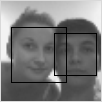
\includegraphics{opencv.png}
    \caption{Detekce obličejů v praxi}
\end{center}
\end{listing}

Algoritmus pro hledání obličejů je použit z knihovny OpenCV a tedy není záměrem
této kapitoly vysvětlovat jej. Byl pouze využit pro ukázku možností e-puck
knihovny.

\subsection{Zdrojový kód}

\begin{mylisting}
\begin{pyc}
#!/usr/bin/env python
# -*- coding: utf-8 -*-

import logging
import time

from Tkinter import *
from ImageTk import PhotoImage

import cv
import ImageDraw
import Image as Img

from epuck.controller import Controller

logging.basicConfig(level=logging.ERROR)

c = Controller('/dev/rfcomm0', timeout=5, asynchronous=True)

# Set camera properties
c.set_front_led(1)
c.set_camera(Controller.GREYSCALE_MODE, 55, 55, 8)

# Create the application layout
root = Tk()
img_face = Label(root)
img_face.pack()

# Load face definitions
cascade = cv.Load('haarcascade_frontalface_alt.xml')

def show_photo():
    # Get the photo
    img = c.get_photo() \
        .get_response() \
        .resize((100, 100), Img.ANTIALIAS)

    # Convert the photo for OpenCV
    cv_img = cv.CreateImageHeader(img.size, cv.IPL_DEPTH_8U, 1)
    cv.SetData(cv_img, img.tostring())

    # Find any faces in the image
    storage = cv.CreateMemStorage(0)
    cv.EqualizeHist(cv_img, cv_img)
    faces = cv.HaarDetectObjects(cv_img, 
                cascade, 
                storage, 
                1.2, 2,
                cv.CV_HAAR_DO_CANNY_PRUNING)

    if faces:
        for f in faces:
            # Draw a border around a found face.
            draw = ImageDraw.Draw(img)
            draw.setfill(0)
            draw.rectangle([(f[0][0],
                             f[0][1]),
                            (f[0][0] + f[0][2],
                             f[0][1] + f[0][3])])

    # Show the image with faces
    image = PhotoImage(img)
    img_face.config(image=image)
    img_face.img = image

    # Run this function again in 10ms
    img_face.after(10, show_photo)

# Get first photo and run the main loop
show_photo()
root.mainloop()
\end{pyc}
\captionof{listing}{Grafická aplikace pro detekci obličejů}
\label{opencv}
\end{mylisting}

\subsection{Vysvětlení programu}

Program se skládá z několika částí, které využívají jednotlivé knihovny, na
začátku (zdrojový kód \ref{kamera_okno}) je třeba nastavit kameru robota. Pro
detekci obličejů se používá černobílých fotek, takže bylo možné zvětšit
velikost fotografie. Dále je nutné vytvořit grafické okno pomocí knihovny
Tkinter a načíst data pro knihovnu OpenCV, která používá pro detekci obličejů.

\begin{listing}
\begin{pyc*}{firstnumber=20}
# Set camera properties
c.set_front_led(1)
c.set_camera(Controller.GREYSCALE_MODE, 55, 55, 8)

# Create the application layout
root = Tk()
img_face = Label(root)
img_face.pack()

# Load face definitions
cascade = cv.Load('haarcascade_frontalface_alt.xml')
\end{pyc*}
\caption{Nastavení kamery a vytvoření okna}
\label{kamera_okno}
\end{listing}

Hlavní část je ve funkci \code{show\_photo}, která je pravidelně volána hlavní
smyčkou knihovny Tkinter. V ní pak dochází k zpracování a zobrazení obrázku z
robota. Nejprve (zdrojový kód \ref{photo_resize}) je získána fotka, ta je
následně zvětšena pro lepší prohlížení.

\begin{listing}
\begin{pyc*}{firstnumber=32}
def show_photo():
    # Get the photo
    img = c.get_photo() \
        .get_response() \
        .resize((100, 100), Img.ANTIALIAS)
\end{pyc*}
\caption{Získání fotografie a její zvětšení}
\label{photo_resize}
\end{listing}

Výsledek je převeden do formátu obrázků pro OpenCV. Dále je zavolán algoritmus
pro detekci obličejů, nalezené obličeje jsou zakresleny do fotky (zdrojový kód
\ref{opencv_part}).

\begin{listing}
\begin{pyc*}{firstnumber=38}
    # Convert the photo for OpenCV
    cv_img = cv.CreateImageHeader(img.size, cv.IPL_DEPTH_8U, 1)
    cv.SetData(cv_img, img.tostring())

    # Find any faces in the image
    storage = cv.CreateMemStorage(0)
    cv.EqualizeHist(cv_img, cv_img)
    faces = cv.HaarDetectObjects(cv_img, 
                cascade, 
                storage, 
                1.2, 2,
                cv.CV_HAAR_DO_CANNY_PRUNING)

    if faces:
        for f in faces:
            # Draw a border around a found face.
            draw = ImageDraw.Draw(img)
            draw.setfill(0)
            draw.rectangle([(f[0][0],
                             f[0][1]),
                            (f[0][0] + f[0][2],
                             f[0][1] + f[0][3])])
\end{pyc*}
\caption{Zpracování fotky pomocí OpenCV}
\label{opencv_part}
\end{listing}

Nakonec už je fotka naposledy převedena, tentokrát do formátu pro Tkinter,
a~zobrazena (\ref{tkinter_show}). Funkce \code{after} slouží k periodickému
volání metody \code{show\_photo} každých 10ms. Díky tomu by se měl obraz
aktualizovat téměř v reálném čase (samozřejmě je snímání fotky v robotovi
znatelné na časové prodlevě).

\begin{listing}
\begin{pyc*}{firstnumber=61}
    # Show the image with faces
    image = PhotoImage(img)
    img_face.config(image=image)
    img_face.img = image

    # Run this function again in 10ms
    img_face.after(10, show_photo)
\end{pyc*}
\caption{Převedení a zobrazeni fotky pomocí Tkinter}
\label{tkinter_show}
\end{listing}

